\section{Series Numéricas e Integrales Impropias}

\subsection{Series numéricas}

\begin{defi}
	Una serie de números reales es una pareja de sucesiones de números reales
	$(a_n)_{n \geq 0}$, $(s_n)_{n \geq 0}$, relacionadas por
	\[
		s_n = \sum_{i=0}^{n} a_n
	\]
	Denominaremmos término $n$-ésimo de la serie al elemento $a_n$ y llamaremos
	suma parcial $n$-ésima de la serie a $s_n$
\end{defi}
\begin{obs*}
	Las sumas parciales definen los términos
	\[
		a_0 = s_0 \qquad a_n = s_n - s_{n-1} \quad (n \geq 1)
	\]
\end{obs*}

\begin{defi}
	Llamaremos suma de una serie a
	\[
		s = \lim s_n = \lim\limits_{n \to \infty} \sum_{k=0}^{n} a_n
	\]
	suponiendo que existe
\end{defi}
\begin{obs*}
	Denotaremos $s = \sum\limits_{n \geq 0} a_n = \sum\limits_{n \geq 0}^{\infty} a_n$.
	Esta misma notación nor servirá para representar la serie.
\end{obs*}

\begin{defi}
	Diremos que una serie $\sum a_n$ es convergente o divergente si lo es la
	sucesión de sumas parciales
	\begin{itemize}
		\item convergente \qquad $\lim s_n \in \real$
		\item divergente  \qquad $\lim s_n = \pm \infty$
		\item oscilante \qquad $\nexists \lim s_n$
	\end{itemize}
\end{defi}

\begin{obs}
	Una serie no tiene por qué comenzar por el índice 0, y por tanto, podemos considerar
	series con términos $a_n$ donde $n \geq n_0$. En tal caso, las sumas parciales son
	$s_n = \sum\limits_{k=n_0}^n a_n$, y la suma (si existe) $\sum\limits_{k=n_0}^{\infty}
	a_n = \lim\limits_{n \to \infty} \sum\limits_{k=n_0}^n a_n$.
\end{obs}


\begin{defi}
	Sea $r \in \real$. Llamaremos serie geométrica de razón $r$ a la serie
	\[
		\sum_{n \geq 0} r^n
	\]
\end{defi}

\begin{prop*}
	La serie geométrica es convergente si y solo si $\abs{r} < 1$, en tal caso
	la suma es
	\[
		\sum_{n \geq 0} r^n = \frac{1}{1-r}
	\]
\end{prop*}

\begin{proof}
	Primero, calculamos el término $n$-ésimo
	\[
		s_n = 1 + r + \cdots + r^n = \begin{cases}
			n+1 \qquad \text{si } r = 1 \\
			\frac{r^{n+1} - 1 }{r-1} \qquad \text{si } r \neq 1
		\end{cases}
	\]
	\begin{itemize}
		\item Si $r = 1$, $\lim s_n = \lim\limits_{n  \to \infty} n+1 = \infty$
		\item Si $\abs{r} > 1$, $\lim s_n = \lim\limits_{n \to \infty}
			\frac{r^{n+1} - 1}{r-1} = \infty$
		\item Si $\abs{r} < 1$, $\lim s_n = \lim\limits_{n \to \infty}
			\frac{r^{n+1} - 1}{r-1} = \frac{-1}{r-1}$
		\item Si $r = -1$, $s_n = 0$ si $n$ par y $s_n = 1$ si $n$ impar. Por
			lo tanto la serie es oscilante
	\end{itemize}
\end{proof}

\begin{prop}
	Si $\sum a_n$ es convergente, entonces $\lim a_n = 0$
\end{prop}

\begin{proof}
	Sabemos que $a_n = s_n - s_{n-1}$, por lo tanto
	$\lim a_n = \lim (s_n - s_{n-1})$, como $\lim s_n$ existe (y por lo tanto
	también $\lim s_{n-1}$)
	\[
		\lim a_n = \lim (s_n - s_{n-1}) = \lim s_n - \lim s_{n-1} = 0
	\]
\end{proof}

\begin{prop}[Criterio de Cauchy para series]
	La serie $\sum a_n$ es convergente si $\forall\varepsilon>0$,
	$\exists n_0 \in \n$
	tal que
	\[
		m,n \geq n_0 \implies \abs{s_m - s_n} = \abs{a_m + a_{m-1} \cdots + a_n} <
		\varepsilon
	\]
\end{prop}

\begin{prop}[linealidad]
	Sean $\alpha, \beta \in \real$ y sean $\sum a_n$ y $\sum b_n$ series convergentes.
	Entonces $\sum (\alpha a_n + \beta b_n)$ también lo es y $\sum (\alpha a_n + \beta b_n)
	= \alpha \sum a_n + \beta \sum b_n$.
\end{prop}

\begin{prop}
	Sean dos sucesiones $(a_n)$y $(b_n)$, son iguales salvo en número finito de términos,
	entonces las series $\sum a_n$ y $\sum b_n$ tienen la misma convergencia.
\end{prop}

\begin{proof}
	Sea $d_n = b_n - a_n$, que vale 0 salvo en número finito de términos
	\begin{itemize}
		\item Si $\sum a_n$ converge \qquad $\sum b_n = \sum a_n +
		\overbrace{\sum d_n}^\text{Suma finita}$ $\implies$ $\sum b_n$ converge
		\item Si $\sum a_n$ diverge \qquad $\sum b_n = \sum a_n + \sum d_n
		\implies \sum b_n$ diverge
		\item Si $\sum a_n$ oscila \qquad $\sum b_n = \sum a_n + \sum d_n
		\implies \sum b_n$ oscila
	\end{itemize}
\end{proof}

\begin{prop}[Asociatividad]
	Sea $\sum a_n$ una serie y $(n_k)_{k \geq 0}$ una sucesión estrictamente creciente de
	números naturales. Definimos
	\[
		b_0 = a_0 + \cdots + a_{n_0} \qquad b_k = a_{(n_{k-1}+1)} + \cdots + a_{n_k}
	\]
	Si existe la suma de $\sum a_n$, entonces también existe la suma de $\sum b_k$
	y son iguales.
\end{prop}

\begin{proof}
	Sea $A_n = \sum\limits_{i=0}^{n} a_i$ y $B_k = \sum\limits_{i=0}^{k} b_i$, por la
	definición anterior se tiene que $B_k = A_{n_k}$ y por lo tanto $(B_k)$ es una sucesión
	parcial de $(A_n)$, lo cual implica que si $(A_n)$ converge, $(B_k)$ también
	y lo hace al mismo número.
\end{proof}

%%%%%%%%%%%%%%%%%%%%%%%%%%%%%%%
% SERIES DE NUMEROS POSITIVOS %
%%%%%%%%%%%%%%%%%%%%%%%%%%%%%%%

\subsection{Series de números positivos}

\begin{prop}
	Si una serie $\sum a_n$ es de \textit{términos positivos} ($a_n \geq 0$) entonces la
	sucesión $(s_n)$ de sumas parciales es \textit{creciente}, y por tanto, siempre tiene
	límite:
	\[
		\sum a_n = \lim s_n = \sup_{n \in \n} s_n
	\]
	Este puede ser finito (si la sucesión de sumas parciales es acotada) o infinito (en caso
	contrario).
\end{prop}

\begin{prop}[Criterio de comparación directa]
	Sean $\sum a_n$ y $\sum b_n$ series de términos positivos. Si $\exists n_0$ tal que
	$a_n \leq b_n$ ($\forall n \geq n_0$). Entonces
	\[
		\sum_{n=n_0}^{\infty} a_n \leq \sum_{n=n_0}^{\infty} b_n
	\]
	Por tanto, la convergencia de $\sum b_n$ implica la de $\sum a_n$ y la divergencia de
	$\sum a_n$ implica la de $\sum b_n$.
\end{prop}

\begin{proof}
	Por el enunciado 
	\[
		\sum_{i=n_0}^{n} a_i \leq \sum_{k=n_0}^{n} b_k \implies
		\sum_{i=n_0}^{\infty} a_i \leq \sum_{k=n_0}^{\infty} b_k
	\]
	Los términos $a_0, \cdots, a_{n_0}$ se pueden añadir al sumatorio y no alteran
	la convergencia.
\end{proof}

\begin{defi*}
	Llamamos serie harmónica a la serie
	\[
		\sum_{n \geq 1} \frac{1}{n}
	\]
\end{defi*}

\begin{defi}[Serie de Riemman]
	Sea $p \in \real$. Llamaremos serie harmónica generalizada o serie de Riemman
	de parámetro $p$ a la serie
	\[
		\sum_{n \geq 1} \frac{1}{n^p}
	\]
\end{defi}

\begin{prop*}
	La serie de Riemman es convergente si y solo si $p > 1$.
\end{prop*}

\begin{proof}
	Distinguiremos entre varios casos
	\begin{itemize}
		\item Si $p = 1$. Suponemos que la serie es convergente con suma $s$
		\[
			s = \left( 1 + \frac{1}{2} \right) + \left( \frac{1}{3} + \frac{1}{4}
			\right) + \cdots > \left( \frac{1}{2} + \frac{1}{2} \right) + \left(
			\frac{1}{4} + \frac{1}{4} \right) + \cdots =
			1 + \frac{1}{2} + \frac{1}{3} + \frac{1}{4} + \cdots = s
		\]
		absurdo ya que $s>s$.
		\item Si $p < 1$. 
		\[
			n^p \leq n \implies \frac{1}{n^p} \geq \frac{1}{n}
		\]
		y por comparación directa con la serie harmónica, diverge.
		\item Si $p > 1$.
		\[\begin{split}
			\sum_{n \geq 1} \frac{1}{n^p} = 1 + \left(\frac{1}{2^p} + \frac{1}{3^p}
			\right) + \left( \frac{1}{4^p} + \frac{1}{5^p} + \frac{1}{6^p} +
			\frac{1}{7^p} \right) + \cdots \leq \\ \leq 1 + \left(\frac{1}{2^p} +
			\frac{1}{2^p} \right) + \left( \frac{1}{4^p} + \frac{1}{4^p} +
			\frac{1}{4^p} + \frac{1}{4^p} \right) = 1 + \frac{1}{2^{p-1}} +
			\frac{1}{2^{2(p-1)}} + \cdots
		\end{split}\]
		que es una serie geométrica de razón $\frac{1}{2^{p-1}} < 1$ y por lo tanto
		convergente.
	\end{itemize}
\end{proof}

\begin{prop}[Criterio de comparación en el límite]
	Sean $\sum a_n$ y $\sum b_n$ series de términos estrictamente positivos.
	Suponemos que existe el límite
	\[
		\lim \frac{\sum a_n}{\sum b_n} = l \in [0,+\infty]
	\]
	\begin{itemize}
		\item Si $l < + \infty$. $\sum b_n$ converge $\implies$ $\sum a_n$ converge y
			$\sum a_n$ diverge $\implies \sum b_n$ diverge.
		\item Si $l > 0$. $\sum a_n$ converge $\implies$ $\sum b_n$ converge y si $\sum b_n$
			diverge $\implies \sum a_n$ diverge.
		\item Si $0 < l < +\infty$. Entonces las dos series tienen el mismo caracter.
	\end{itemize}
\end{prop}
\begin{proof}
	Provaremos cada caso de manera individual
	\begin{itemize}
		\item Caso $l < +\infty$. Fijado $\varepsilon > 0$, por definición de límite, existe
		$n_0\in\n$ tal que
		\[
			n \geq n_0 \implies \frac{a_n}{b_n} < l + \varepsilon \implies
			a_n < (l+\varepsilon)b_n
		\]
		y el resultado queda provado por comparación directa.
		\item Caso $l > 0$. Se deduce del primer caso, considerando
		\[
			\lim \frac{b_n}{a_n} = \frac{1}{l}
		\]
		\item Caso $0 < l < +\infty$. Se trata de una conjunción de los casos
		anteriores
	\end{itemize}
\end{proof}

\begin{lema}
	Sea $\sum a_n$ una serie de términos positivos.
	\begin{itemize}
		\item Suponemos que hay $n_0 \in \n$ y $r < 1$ tal que
		\[
			n \geq n_0 \implies a_n^{1/n} < r
		\]
		entonces $\sum a_n < +\infty$
		\item Suponemos que existe $n_0 \in \n$ tal que 
		\[
			n \geq n_0 \implies a_n^{1/n} \geq 1
		\]
		entonces $\sum a_n = +\infty$
	\end{itemize}
\end{lema}

\begin{proof}
	Provaremos cada caso por separado
	\begin{itemize}
		\item $a_n^{1/n} < r \implies a_n < r^n$ que es la serie geométrica de
		razón $r < 1$, de modo que por comparación directa el resultado queda
		demostrado.
		\item $a_n^{1/n} \geq 1 \implies a_n \geq 1$ y por lo tanto diverge.
	\end{itemize}
\end{proof}

\begin{prop}[Criterio de la raíz de Cauchy]
	Sea $\sum a_n$ una serie de términos positivos. Suponemos que existe
	$\lim a_n^{1/n} = \alpha$, entonces, si $\alpha > 1$ la serie diverge y si
	$\alpha < 1$ la serie converge.
\end{prop}

\begin{proof}
	Demostraremos cada caso por separado
	\begin{itemize}
		\item Caso $\alpha < 1$. Sea $\alpha < r < 1$. Existe $n_0 \in \n$ tal que
		\[
			n \geq n_0 \implies a_n^{1/n} \leq r
		\]
		Y el resultado queda provado aplicando el lema anterior.
		\item Caso $\alpha > 1$. Existe $n_0 \in \n$ tal que
		\[
			n \geq n_0 \implies a_n^{1/n} \geq 1
		\]
		y aplicamos el lema anterior.
	\end{itemize}
\end{proof}

\begin{lema}
	Sea $\sum a_n$ una serie de términos estrictamente positivos.
	\begin{itemize}
		\item Suponemos que hay $n_0 \in \n$ y $r < 1$ tal que 
		\[
			n \geq n_0 \implies \frac{a_{n+1}}{a_n} \leq r
		\]
		entonces $\sum a_n < + \infty$
		\item Suponemos que existe $n_0 \in \n$ tal que
		\[
			n \geq n_0 \implies \frac{a_{n+1}}{a_n} \geq 1
		\]
		entonces $\sum a_n = + \infty$
	\end{itemize}
\end{lema}

\begin{proof}
	Separaremos los casos.
	\begin{itemize}
		\item 
		\[
			\frac{a_n+1}{a_n} \leq r \implies a_{n+1} \leq r a_n \implies a_n \leq
			C r^n \quad (n \geq n_0)
		\]
		donde $C = \frac{a_{n_0}}{r^{n_0}}$ y por el criterio de comparación
		directa $\sum a_n$ converge.
		\item $\frac{a_{n+1}}{a_n} \geq 1\implies a_{n+1} \geq a_n \implies a_n$ es creciente
			$\implies \sum a_n$ diverge
	\end{itemize}
\end{proof}

\begin{prop}[Criterio del cociente de Alembert]
	Sea $\sum a_n$ una serie de términos estrictamente positivos. Suponemos que existe
	$\lim \frac{a_{n+1}}{a_n} = \alpha$, entonces
	\begin{itemize}
		\item Si $\alpha > 1$ la serie diverge
		\item Si $\alpha < 1$ la serie converge
	\end{itemize}
\end{prop}

\begin{proof}
	Separamos los dos casos
	\begin{itemize}
		\item Si $\alpha < 1$. Sea $\alpha < r < 1$ entonces $\exists n_0 \in \n$
		tal que
		\[
			n \geq n_0 \implies \frac{a_{n+1}}{a_n} \leq r
		\]
		y aplicamos el lema anterior.
		\item Si $\alpha > 1$. Entonces  $\exists n_0 \in \n$ tal que
		\[
			n \geq n_0 \implies \frac{a_{n+1}}{a_n} \geq 1
		\]
		y aplicamos el lema anterior.
	\end{itemize}
\end{proof}

\begin{example*}
	Estudiar la convergencia de 
	\begin{itemize}
		\item $\sum\limits_{n \geq 0} \frac{1}{n!}$. \\
			$n!$ crece más que	$n^2$ ($n! > n^2$) $\implies \frac{1}{n!} < \frac{1}{n^2}$
			que es la serie de Riemman de parámetro 2 (convergente). Por tanto,
			$\sum\limits_{n \geq 0}^\infty \frac{1}{n!}$ es convergente.
		\item $\sum \frac{x^n}{n!}$ para $x > 0$. \\
			\[
				\lim_{n \to \infty} \frac{\frac{x^{n+1}}{(n+1)!}}{\frac{x^n}{n!}} = 
				\lim_{n \to \infty} \frac{x^{n+1}n!}{x^n(n+1)n!} = \lim_{n \to \infty}
				\frac{x}{n+1} = 0 < 1
			\]
			Por lo tanto, aplicando el criterio del cociente de Alembert, la serie coverge.
		\item $\sum \alpha^{n+\sqrt{n}}$ \\
			\[
				\lim_{n \to \infty} \alpha^{\frac{n + \sqrt{n}}{n}} =
				\lim_{n \to \infty} \alpha^{1 + \frac{1}{\sqrt{n}}} = \alpha
			\]
			Por lo tanto, por el criterio de la raíz, $\begin{cases} \alpha < 1
			\text{ convergente} \\ \alpha > 1 \text{ divergente}\end{cases}$. Si $\alpha =1$,
			la serie es $\sum 1^{n + \sqrt{n}} = \sum 1$ que es divergente.
	\end{itemize}
\end{example*}

\begin{obs}
	Los criterios anteriores no deciden cuando $\alpha = 1$. Como $\sfrac{a_{n+1}}{a_n} \to
	\alpha$ implica que $a_n^{\sfrac{1}{n}} \to \alpha$, si el criterio del cociente no
	decide, entonces el de la raíz tampoco.
\end{obs}

\begin{prop}[Criterio de Raabe]
	Sea $\sum a_n$ una serie de términos estrictamente positivos tal que existe el límite
	\[
		L = \lim_{n \to \infty} n\left( 1 - \frac{a_{n+1}}{a_n} \right)
	\]
	Si $L > 1$, la serie $\sum a_n$ es convergente. Si $L < 1$, la serie $\sum a_n$ es
	divergente.
\end{prop}

\begin{prop*}[Criterio de condensación]
	Sea $(a_n)$ una sucesión de números positivos decreciente. Entonces
	\[
		\sum_{n=0}^{\infty} a_n \text{ converge} \iff \sum_{n=0}^{\infty} 2^n a_{2^n}
		\text{ converge}
	\]
\end{prop*}

\begin{prop*}[Criterio logarítmico]
	Sea $\sum a_n$ una serie de términos positivos tal que existe el límite
	\[
		L = \lim_{n \to \infty} \frac{- \ln(a_n)}{\ln(n)} = \lim_{n \to \infty}
		\frac{\ln\left( \frac{1}{a_n} \right)}{\ln(n)}
	\]
	Si $L > 1$, la serie $\sum a_n$ es convergente. Si $L < 1$, la serie $\sum a_n$ es
	divergente.
\end{prop*}

\begin{prop}[Criterio de la integral]
	Sea $n_0 \in \n$ y $f \colon [n_0, +\infty) \to \real$ positiva, localmente integrable
	y decreciente. Consideramos $a_n = f(n)$ ($n \geq n_0$) entonces
	\begin{enumerate}[i)]
		\item La serie $\sum a_n$ y la integral impropia
		$\int_{n_0}^{+\infty} f$ tienen el mismo carácter.
		\item Para $N \geq n_0$
		\[
			\sum_{n \geq n_0}^{\infty} a_n = \sum_{n = n_0}^{N-1} + \int_{N}^{+\infty}f +
			\varepsilon_n
		\]
		donde $\varepsilon_n \in [0, a_n]$
	\end{enumerate}
\end{prop}

\begin{example*}
	\begin{itemize}
		\item[]
		\item $\sum \frac{1}{n^\alpha}$ tiene el mismo carácter que
			$\int_{1}^{\infty} \frac{1}{x^\alpha} \dif x$ (convergete $\iff \alpha > 1$)
		\item Calcular $\sum\limits_{n\geq 1} \frac{1}{n^{1.01}}$ con error $< 10^{-3}$. \\
			Necesitamos que
			\[
				\frac{1}{N^{1.01}} < 10^{-3} \implies N > 1000^{\sfrac{1}{1.01}} \implies
				N \geq 934
			\]
			Calculamos ahora
			\[
				\sum_{n=1}^{933} \frac{1}{n^{1.01}} + \int_{934}^{+\infty}
				\frac{\dif x}{x^{1.01}} \simeq 100.577 \simeq\sum_{n\geq 1}\frac{1}{n^{1.01}}
			\]
	\end{itemize}
\end{example*}

\begin{prop}
	Sea $\sum a_n$ una serie de términos positivos. Dada cualquier permutación $\sigma
	\colon \n \to \n$, la serie $\sum a_{\sigma(n)}$ tiene la misma suma que $\sum a_n$.
\end{prop}

\begin{proof}
	Sea $A_n = \sum\limits_{k=0}^n a_k$ y $B_n = \sum\limits_{k=0}^n a_{\sigma(k)}$ y sean
	$A = \lim A_n$ y $B = \lim B_n$. Sea
	$m \in \n$, entonces $\exists n \in \n$ tal que
	\[
		\setb{0,1, \dots, m} \leq \setb{\sigma(0), \sigma(1), \dots, \sigma(n)}
	\]
	ya que $\sigma$ es suprayectiva. Entonces $a_0 + a_1 + \cdots + a_m \leq a_{\sigma(0)} + 
	a_{\sigma(1)} + \cdots + a_{\sigma(n)}$ por lo tanto, $A_m \leq B_n \implies A \leq B$.
	Haciendo el mismo razonamiento para $\inv{\sigma}$ (biyectiva), obtenemos que $B \leq A$.
	Y por lo tanto, $A = \sum a_n = \sum a_{\sigma(n)} = B$.
\end{proof}

\subsection{Series absolutamente convergentes y condicionalmente convergentes}

\begin{defi}
  Diremos que una serie $\sum a_n$ es absolutamente convergente, si la serie $\sum \abs{a_n}$ es convergente.
\end{defi}

\begin{prop}
  Toda serie absolutamente convergete es convergente.
\end{prop}

\begin{proof}
  Aplicamos criterio de Cauchy para series a $\sum \abs{a_n}$: $\forall \varepsilon > 0$ $\exists n_0 \in \n$
  tal que
  \[
    m > n \geq n_0 \implies \abs{\abs{a_{n+1}} + \cdots + \abs{a_m}} < \varepsilon \implies
    \abs{a_{n+1}} + \cdots + \abs{a_m} < \varepsilon
  \]
  De donde se deduce que
  \[
    \abs{a_{n+1} + \cdots + a_n} < \abs{a_{n+1}} + \cdots + \abs{a_m} < \varepsilon
  \]
  (por la desigualdad triangular). Y por lo tanto, $\sum a_n$ cumple el criterio de Cauchy.

\end{proof}

\begin{defi}
  Una serie convergente, que no es absolutamente convergente, se dice que es condicionalmente convergente.
\end{defi}

\begin{example*}
  La serie armónica alternada $\sum \frac{(-1)^n}{n}$ es condicionalmente convergente.
\end{example*}

\begin{defi}
  Sea $a \in \real$. Definimos $a_+$ (la parte positiva de $a$) como $a_+ = \max(a, 0)$, asimismo, definimos
  la parte negativa de $a$ como $a_- = \max(-a,0)$.
\end{defi}

\begin{obs*}
  Dado un $a$, podemos expresar $a = a_+ - a_-$ y $\abs{a} = a_+ + a_-$
\end{obs*}

\begin{obs*}
  Dada $f \colon X \to \real$, podemos hacer exactamente lo mismo, ($f = f_+ - f_-$, $\abs{f} = f_+ + f_-$)
\end{obs*}

\begin{example*} \hspace{0pt}
  \begin{center}
  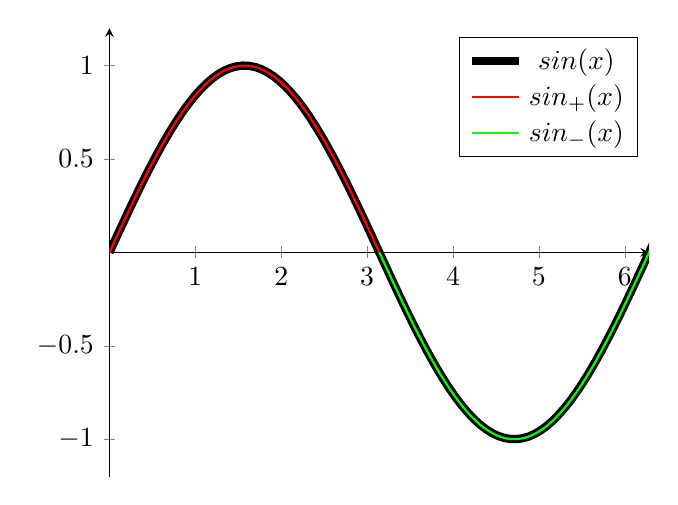
\begin{tikzpicture}
  \begin{axis}[
    xmin = 0,
    xmax = 2*3.14151625,
    ymin = -1.2,
    ymax = 1.2,
    samples = 100,
    axis lines = center
  ]
    \addplot[domain=0:7,line width=3pt]{sin(deg(x))};
    \addplot[domain=0:3.14151625,color=red,thick]{sin(deg(x))};
    \addplot[domain=3.14151625:7,color=green,thick]{sin(deg(x))};
    
    \legend{$sin(x)$,$sin_+(x)$,$sin_-(x)$}
  \end{axis}
  \end{tikzpicture}
  \end{center}
  
\end{example*}

\begin{lema}
  Sea $(a_n)$ una sucesión de números reales. Sean $(p_n)$ y $(q_n)$ sus partes positiva y negativa
  (respectivamente).
  \begin{enumerate}[i)]
    \item $\sum a_n$ converge absolutamente $\iff$ $\sum p_n$, $\sum q_n$ son convergentes.
    \item Si $\sum a_n$ es condicionalmente convergente, entonces $\sum p_n$ y $\sum q_n$ son divergentes
  \end{enumerate}

\end{lema}


